\section{The Dynamic Barrier as a Local Differential Horizon}
\label{sec:dynamic_barrier}

\subsection{From Phenomenological Barrier to Dynamic Feedback}

The earlier use of a $\kappa_B$ barrier term should be read as a
phenomenological approximation.
It records that complete closure is resisted,
but it does not explain why the resistance exists.
In schematic form the previous description was
\begin{equation}
  B(L)=-\kappa_B\ln\left(1-\frac{L}{L_{\max}}\right),
\end{equation}
so that the resistance diverges as $L$ approaches $L_{\max}$.

This section replaces that interpretation.
The barrier is not introduced as an external prohibition.
It is generated by the same motion that attempts to close the system:
closure increases the velocity of closure,
closure velocity generates rotational feedback,
and rotational feedback bends the trajectory away from complete
closure.

The resulting model is a local spacetime-side realization of
Proposition 1 of the \DHP{}.
Complete closure, $L=1$, corresponds not to an ordinary state inside
the model,
but to the boundary at which no internal difference remains available
to sustain the generated description---the local signature of the
\ungenerated{} domain.
The model does not allow this limit to be reached from outside
by imposing a wall.
It shows how the approach to that limit becomes dynamically unstable
from within the coupled motion of closure, rotation, and dissipation.

\medskip
\begin{quote}
Complete closure is not prohibited by a wall.\\
Rather, motion toward complete closure destabilizes its own existence.
\end{quote}
\medskip

Let $q$ be an unconstrained closure coordinate and define
\begin{equation}
  L=\frac{1}{1+\exp(-q)} .
\end{equation}
The dynamics are
\begin{equation}
  \frac{dq}{dt}=v ,
\end{equation}
\begin{equation}
  \frac{dv}{dt}
  =
  AL
  -
  B\Omega^2L
  -
  Dv ,
\end{equation}
and
\begin{equation}
  \frac{d\Omega}{dt}
  =
  CLv
  -
  E\Omega .
\end{equation}
Here $v$ is closure velocity and $\Omega$ is the rotational or
vortical feedback generated by closure motion.
There is no explicit $\kappa_B$ potential term.
If a barrier appears, it must appear as a dynamical effect of the
coupling among $L$, $v$, and $\Omega$.

\subsection{Fixed Points and the Degenerate Manifold}

The near-closure balance is easiest to see in the conserved-rotation
limit $E=0$.
For $L\simeq1$ and $B>0$, the closure acceleration is approximately
\begin{equation}
  \frac{dv}{dt}
  \simeq
  A
  -
  B\Omega^2
  -
  Dv .
\end{equation}
The closure drive is balanced when
\begin{equation}
  \Omega\simeq\sqrt{\frac{A}{B}},
  \qquad
  v\simeq0 .
\end{equation}

More exactly, in the full three-variable system with $E=0$,
the fixed-point condition gives $v^*=0$,
while $\Omega^*$ is not forced to vanish by rotational dissipation.
The remaining condition is
\begin{equation}
  L^*\left(A-B(\Omega^*)^2\right)=0 .
\end{equation}
For $L^*>0$, this yields
\begin{equation}
  \Omega^*=\sqrt{\frac{A}{B}},
\end{equation}
while $L^*$ itself remains undetermined.
Thus the conserved-rotation limit contains a one-dimensional
fixed-point manifold
\begin{equation}
  \left\{ \left(L,0,\sqrt{\frac{A}{B}}\right) : L\in(0,1) \right\}.
\end{equation}
This degeneracy is lifted by any $E>0$,
which selects the asymptotic near-closure branch instead of leaving
$L$ neutral.

In this projection the system appears to approach rest.
However, this apparent rest does not mean that the system has reached
complete closure.
It means that the observable closure velocity has been balanced by
rotational self-resistance.

This distinction matters.
The sigmoid map guarantees $0<L<1$ for finite $q$,
while the formal limit $L=1$ requires $q\to\infty$.
The degenerate endpoint is therefore not an ordinary point in the
finite state space.
It is the boundary at which the generated description would lose the
difference needed to describe its own generation.
The dynamic barrier is the local trace of this boundary inside the
finite dynamics.

\subsection{The Collapse of the Critical Dissipation Interpretation}

Previous scans identified a numerical threshold
\begin{equation}
  D_c\approx0.0875
\end{equation}%
\begin{NoHyper}\footnote{%
The numerical value depends on the empirical instability threshold
used to define relaxation in a finite observation window.
For the criterion $I(D)<\theta$,
repeating the analysis on the same integration data with
$\theta\in\{0.01,0.02,0.03,0.05,0.07,0.10\}$
gives $D_c(\theta)\in[0.075,0.125]$.
This dependence is not a defect of the interpretation;
it is evidence that $D_c$ is a finite-window relaxation threshold,
not a sharp bifurcation point.%
}\end{NoHyper}
in the case $E=0$.
That value remains diagnostically useful,
but its interpretation must be weakened.
It should not be read as a true bifurcation or as a universal dynamical
critical point.
It is a finite-window relaxation threshold:
above this value the selected observation window sees the trajectory
relax rapidly enough to appear quasi-closed,
whereas below it the same window continues to resolve persistent
phase rotation.

This reinterpretation is not a retreat from the barrier argument.
It clarifies it.
The question is not whether a single scalar threshold separates
structure from non-structure absolutely.
The question is whether a spacetime-generated model can reach the
absence of difference from within its own finite coordinates.
The observed answer is negative.
Changing the window may change the apparent relaxation threshold,
but it does not turn the formal closure endpoint into an attainable
state.

\subsection{Additional Observation Windows}

The following diagnostics use the same ODE system.
They are observation windows, not new physical variables.
Their purpose is to test whether apparent convergence in one projection
is equivalent to genuine disappearance of motion.
In other words,
convergence and dispersal can produce the same appearance when the
observation window is too narrow to distinguish them.
The point is methodological:
if a claim of rest disappears when the same trajectory is viewed
through a richer reconstruction,
then the rest was not an absolute state but a projection-dependent
description.

Figure~\ref{fig:barrier_window_phase_spiral} plots the conserved
rotation case in the centered plane
$(v,\Omega-\sqrt{\frac{A}{B}})$.
Even when the amplitude decays, the trajectory retains phase rotation
around the closure-balance point.
Thus apparent convergence depends on the observation window:
a scalar closure plot can look nearly static while the phase projection
still displays rotation.

\begin{figure}[htbp]
  \centering
  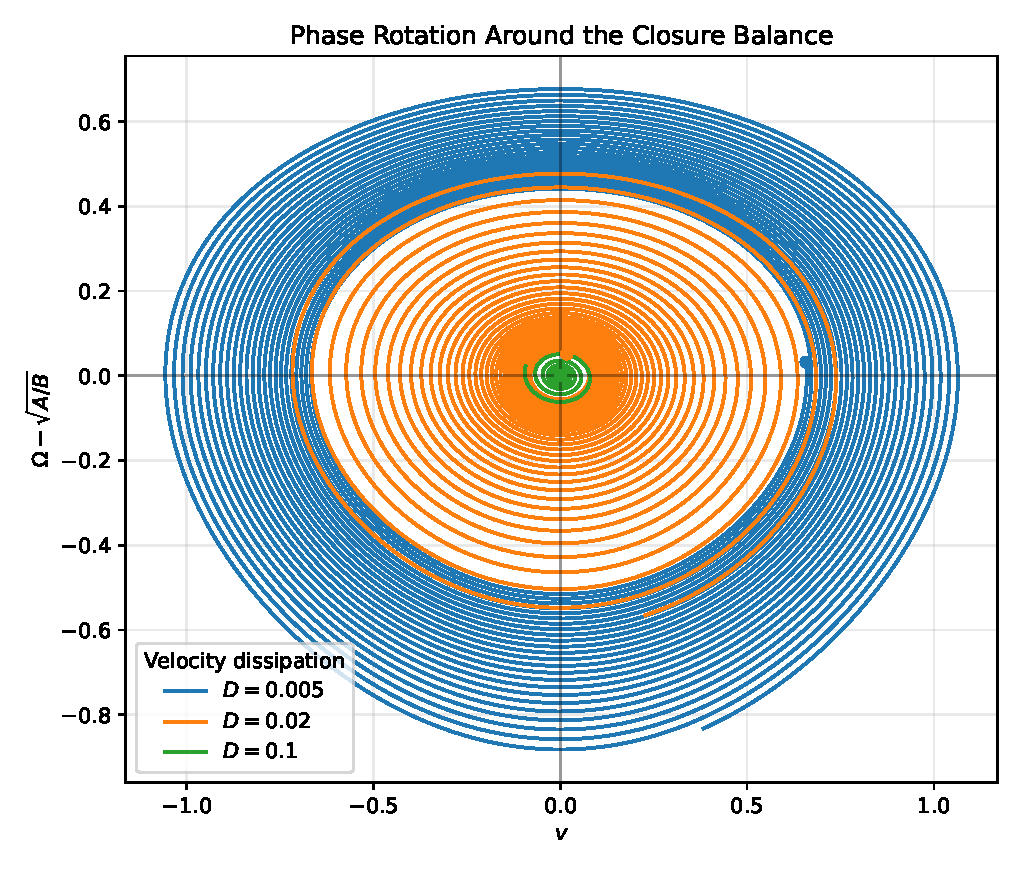
\includegraphics[width=\linewidth]{figures/fig_barrier_window_01_phase_spiral.pdf}
  \caption{%
    Phase rotation around the near-closure balance in the conserved
    rotational-energy limit.
    The radius decays under dissipation,
    but phase rotation remains visible in the centered projection.
  }
  \label{fig:barrier_window_phase_spiral}
\end{figure}

The sliding-window extent in
Fig.~\ref{fig:barrier_window_extent_decay} shows approximately
exponential relaxation over finite windows.
This supports the reinterpretation of $D_c$ as a finite-window
relaxation threshold rather than a sharp dynamical critical point.

\begin{figure}[htbp]
  \centering
  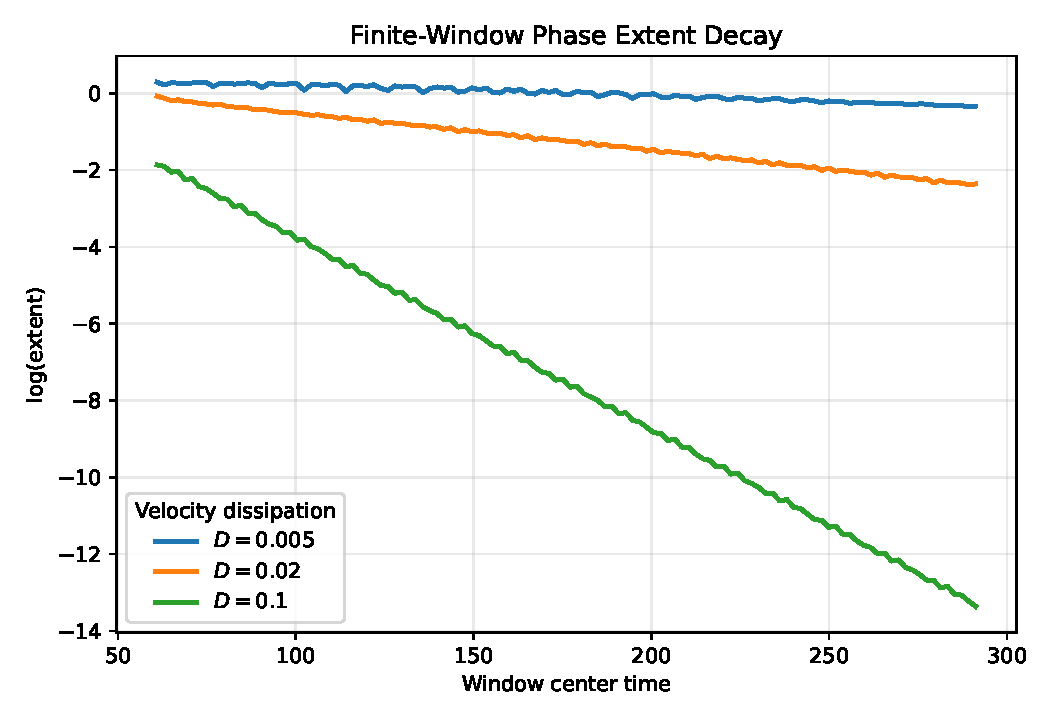
\includegraphics[width=\linewidth]{figures/fig_barrier_window_02_extent_decay.pdf}
  \caption{%
    Finite-window decay of phase-space extent under velocity
    dissipation.
    The approximately linear trend in log scale supports the
    relaxation-threshold interpretation.
  }
  \label{fig:barrier_window_extent_decay}
\end{figure}

The spectrum of $v(t)$ in
Fig.~\ref{fig:barrier_window_spectrum}
shows a fundamental frequency together with harmonic structure:
the dominant peaks appear at harmonically related frequencies rather
than as a featureless decay of spectral power.
These peaks are generated by the nonlinear sigmoid closure map and
the quadratic feedback term $B\Omega^2L$.
They show that the near-closure state is not reducible to a single
static scalar value.

\begin{figure}[htbp]
  \centering
  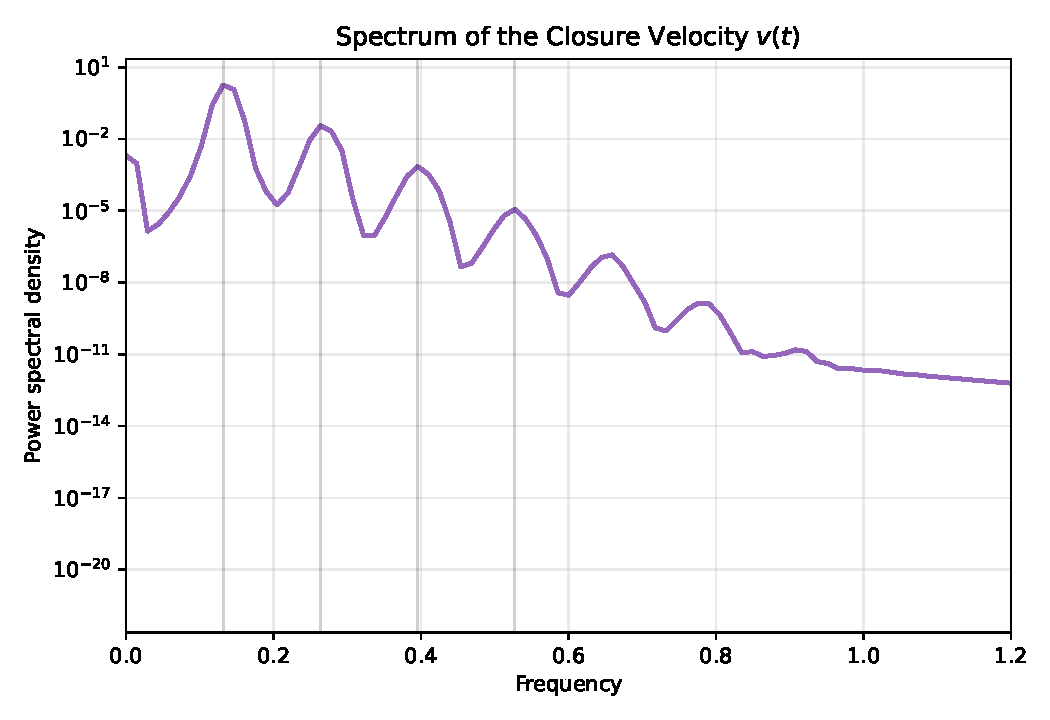
\includegraphics[width=\linewidth]{figures/fig_barrier_window_03_spectrum.pdf}
  \caption{%
    Spectral content of closure velocity generated by nonlinear
    feedback.
    Dominant peaks occur at harmonically related frequencies.
  }
  \label{fig:barrier_window_spectrum}
\end{figure}

Figures~\ref{fig:barrier_window_delay_embedding}
and~\ref{fig:barrier_window_high_derivative}
make the same point in reconstructed state spaces.
The delay embedding of $v(t)$ and the higher-derivative projection
show that what appears as rest in one window reappears as motion in
another.
The trajectory is therefore not exhausted by the scalar statement
``$v$ becomes small.''

\begin{figure}[htbp]
  \centering
  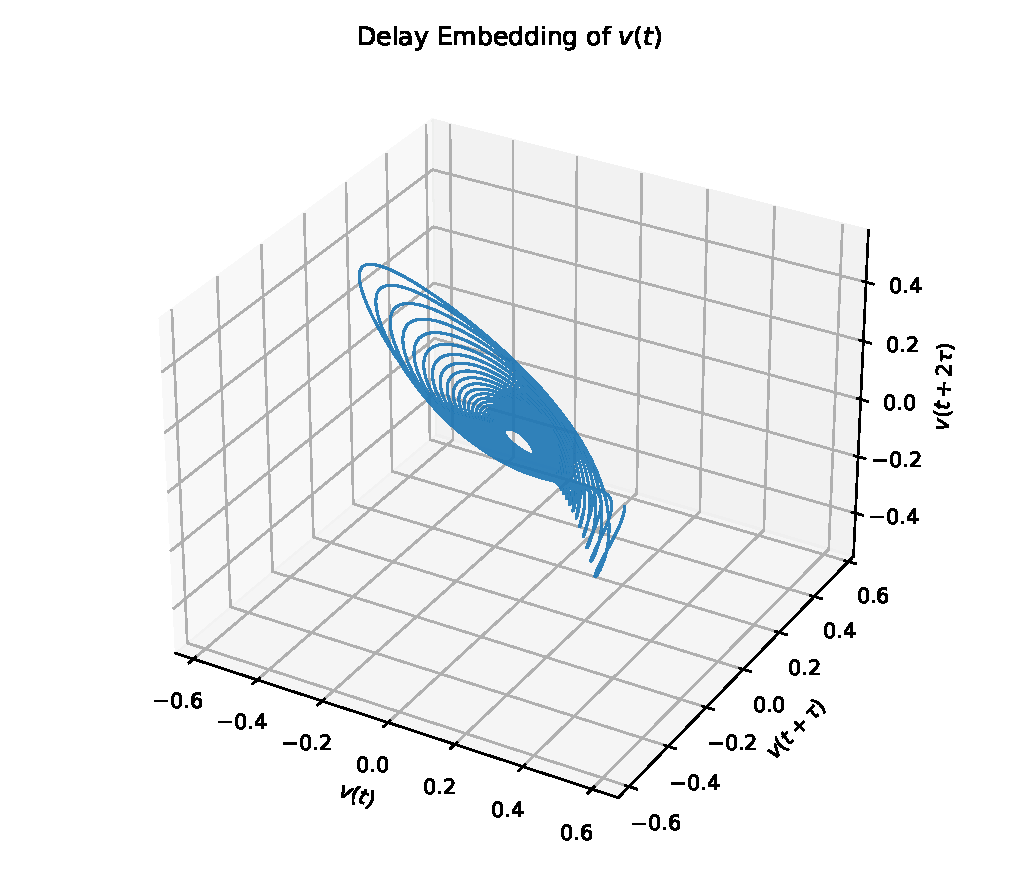
\includegraphics[width=\linewidth]{figures/fig_barrier_window_04_delay_embedding.pdf}
  \caption{%
    Delay embedding of closure velocity as an observation-window
    reconstruction.
    The reconstructed loop shows motion hidden by scalar convergence.
  }
  \label{fig:barrier_window_delay_embedding}
\end{figure}

\begin{figure}[htbp]
  \centering
  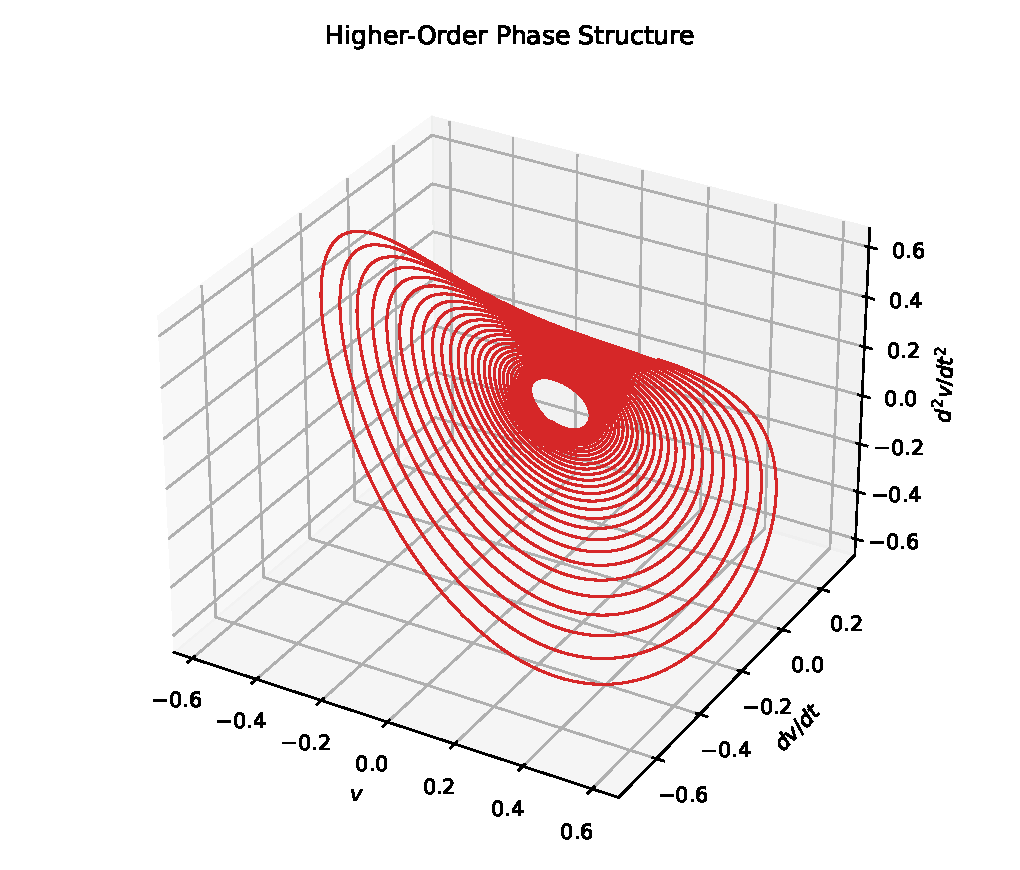
\includegraphics[width=\linewidth]{figures/fig_barrier_window_05_high_derivative_space.pdf}
  \caption{%
    Higher-order phase structure in closure-velocity derivatives.
    Small projected motion reappears as curvature in derivative space.
  }
  \label{fig:barrier_window_high_derivative}
\end{figure}

Finally, Fig.~\ref{fig:barrier_window_envelope_spectrum}
examines the residual spectrum of the detrended radial envelope
\begin{equation}
  r(t)=\sqrt{v(t)^2+\left(\Omega(t)-\sqrt{\frac{A}{B}}\right)^2}.
\end{equation}
The envelope itself contains modulation.
Its residual spectrum again displays dominant peaks at harmonically
related frequencies, now in the decay envelope rather than directly in
$v(t)$.
This confirms that the apparent barrier is not a static potential wall;
it is a delayed rotational self-resistance whose signatures depend on
how the motion is observed.

\begin{figure}[htbp]
  \centering
  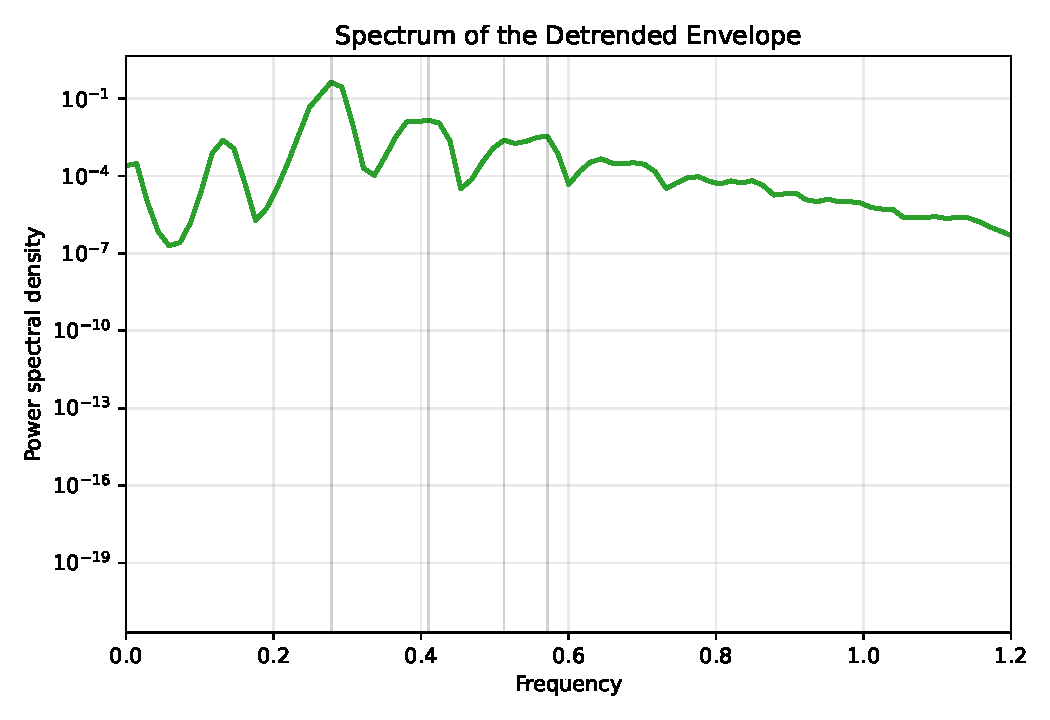
\includegraphics[width=\linewidth]{figures/fig_barrier_window_06_envelope_spectrum.pdf}
  \caption{%
    Residual spectrum of the detrended phase-envelope radius.
    Envelope modulation remains after the dominant decay is removed.
  }
  \label{fig:barrier_window_envelope_spectrum}
\end{figure}

\subsection{Apparent Rest as a Projection}

The phrase ``quasi-closure'' should therefore be understood carefully.
It does not mean that the system has reached a final static object.
It means that, in a selected finite observation window,
the closure coordinate, closure velocity, rotational feedback,
and dissipative losses have entered a coherent balance.

This balance is projection-dependent.
In the $L(t)$ projection, the system may appear nearly closed.
In the $(v,\Omega-\sqrt{\frac{A}{B}})$ projection, it may still rotate.
In a delay embedding, the same signal can retain a loop-like structure.
In derivative space, small motion can reappear as higher-order
curvature.

This is not only a numerical artifact of plotting.
At finite $q$ the sigmoid map is analytic,
so a local expansion of $L(q)$ contains higher powers of the closure
coordinate.
Together with the quadratic feedback term $B\Omega^2L$,
these nonlinearities mix frequencies and generate harmonic content.
The apparent rest of the scalar closure coordinate can therefore
coexist with residual motion in richer reconstructions.

The observation windows form a hierarchy.
Each window suppresses some components of the trajectory while exposing
others.
Adding a phase portrait, a spectrum, a delay embedding,
or a derivative-space reconstruction does not add new physics;
it asks whether the same finite trajectory still contains difference
after a narrower projection has declared it to be at rest.

The dynamic barrier is therefore not a hidden external wall.
It is the condition under which closure can remain describable without
erasing the difference required for description.
Dissipation does not destroy structure.
It determines whether the remaining motion can be organized as
quasi-closure rather than persisting as unresolved rotation.

\subsection{The Dynamic Barrier as a Local Differential Horizon}

The revised interpretation is the following.
The dynamic barrier is not merely a resistance term preventing complete
closure.
It is the internal signature of a descriptive boundary:
a spacetime-generated model cannot reach the absence of difference
from which spacetime itself is generated.

In this sense, the barrier is a local \DH{}.
It is not the global statement of the \DHP{} itself,
but a finite dynamical model of how Proposition 1 appears from within
a generated description.
The model does not prove the \DHP{} from mechanics.
Rather, it shows the spacetime-side form of the same limitation:
the attempt to remove all difference generates dynamics that prevent
the removal from being completed inside the model.

The previous $\kappa_B$ term can therefore be retained only as an
effective phenomenological shorthand.
In a stable quasi-closure regime,
and only in a projected or coarse-grained sense,
one may write
\begin{equation}
  \kappa_B^{\mathrm{eff}}\sim\Omega^2 ,
\end{equation}
but this is not a fundamental potential.
It is a projected measure of delayed rotational self-resistance.

\medskip
\begin{quote}
\VED{} does not impose non-closure as an external law.\\
It derives non-closure as the only dynamically coherent regime
capable of sustaining structure.
\end{quote}
\medskip

Complete closure would remove the difference by which the model
describes its own generation.
For that reason it is not reached as an ordinary dynamical endpoint.
It appears instead as a local Differential Horizon:
the boundary at which a spacetime-generated description can no longer
complete its own closure from within.
This makes Section~\ref{sec:dynamic_barrier} not a peripheral
application of the broader framework,
but its smallest form:
the structure of the \DHP{},
made local enough to be solved as a finite ODE.
